\chapter{Implementação}
\label{cap:implementation}

Neste capítulo apresentamos a implementação da biblioteca cliente HTTP/2, denominada http2, em termos da capacidade exigida pela especificação do HTTP/2 e com as características dos modelos de programação orientada a eventos e programação concorrente em Lua, realizando os conceitos e ideias apresentados no Capítulo \ref{cap:theory}. Serão identificadas as restrições da implementação que foram importantes em orientar as decisões de projeto durante o processo de desenvolvimento e o impacto dessas restrições. A implementação também será descrita em um nível maior de detalhes, no qual códigos que são críticos para a operação da biblioteca serão apresentados. Também mostraremos os problemas que surgiram durante a implementação e como lidamos com eles.

\section{Modelo de Eventos}
\label{cap:events}

O modelo de programação orientado a eventos foi adotado na implementação da biblioteca http2. Nesse modelo, um {\em loop} principal denominado {\em loop de eventos} fica responsável por receber eventos e despachá-los para seus respectivos tratadores, normalmente representadas por funções {\em callbacks}. Assim que um evento é alcançado, o fluxo de execução é transferido para a {\em callback}, fazendo com que a execução só retorne ao {\em loop} quando o processamento da {\em callback} chegar ao fim ou quando o fluxo da execução ser explicitamente devolvido. Nenhum novo evento será recebido e processado enquanto o {\em loop} não estiver executando novamente, ou seja, enquanto a {\em callback} não transferir o controle de volta para o {\em loop}.

Essa decisão foi tomada porque o diagrama de transição de estados da Figura \ref{fig:ciclo_fluxo} se assemelha bastante com a programação orientada a eventos. Internamente pode existir uma constante mudança no estado do cliente HTTP/2 com base nos fluxos recebidos e processados. Um fluxo se encontra em um estado, que é modificado com a chegada de um novo evento. Esse evento pode ser, por exemplo, o recebimento de um quadro do tipo {\em HEADERS} ou o envio desse mesmo quadro. Como resultado, o modelo de programação orientada a eventos foi empregado para implementar o ciclo de vida de um fluxo.

Em reflexo do funcionamento do ciclo de vida de um fluxo e pelo fato de cada requisição enviada por um cliente HTTP/2 ser associada a um fluxo, toda a implementação da biblioteca http2 segue o modelo orientado a eventos, não só para as características internas de baixo nível do protocolo HTTP/2 mas também para a exposição e controle da API disponibilizada junto com a biblioteca (ver Seção \ref{sec:api}). Apesar disso, um programador que utiliza a biblioteca http2 não precisa saber sobre o ciclo de vida de fluxos porque o trabalho de controlar esse ciclo é realizado internamente pela biblioteca.

Nesse contexto, as características de {\em multithreading} cooperativa de Lua descritas na Seção \ref{subsec:coroutines} simulam bem o modelo de orientação a eventos. As {\em callbacks} podem ser implementadas como {\em threads} cooperativas e têm como opção devolver o fluxo de execução ao {\em loop} sem necessariamente terminar o tratamento completo do evento. Durante o processamento das {\em callbacks}, elas conseguem transferir o controle de volta ao {\em loop} e esperar a ocorrência de um evento requerido para que a execução venha a ser retomada.

Esse modelo de eventos é comumente escolhido no cenário de programação de aplicações de rede. Em Lua, poderíamos utilizar co-rotinas diretamente para implementar esse modelo, em que teríamos que chamar funções da biblioteca padrão {\em coroutine} como forma alternativa de implementar o modelo de eventos. Porém, durante a implementação, focamos em utilizar todas as facilidades de escalonamento de co-rotinas da biblioteca Copas \cite{Copas} de forma a gerenciar co-rotinas mais facilmente.

A biblioteca Copas descrita na Seção \ref{subsec:copas} pode cumprir o papel de programar eventos porque ela possui funções que permitem escalonar {\em threads}. O diagrama de sequência UML na Figura \ref{fig:events} mostra como Copas foi aproveitada como a entidade responsável por escalonar {\em threads} e foi feita com base no comportamento de tratamento de eventos com {\em multithreading} cooperativa mostrado por Silvestre \cite{silvestre2009modelos}.

Uma nova {\em thread} cooperativa é criada para tratar o evento A e transfere o controle imediatamente para a mesma. Após algum processamento, a {\em thread} termina o processamento do evento A, finaliza sua execução e o controle é devolvido ao {\em copas.loop()}, que por sua vez recebe um novo evento B. Mas o evento B não é processado por completo, devolvendo o controle para o {\em copas.loop()} imediatamente após a chamada de {\em copas.sleep(-1)}. Novamente com o controle, o {\em copas.loop()} recebe um terceiro evento C, que continua a processar o evento B através da {\em thread} B. Observe que a execução do {\em copas.loop()} não é necessariamente interrompida após a chamada de {\em copas.wakeup()}. Dependendo das próximas instruções a serem executadas pelo {\em copas.loop()}, ele continuará executando até que alguma chamada de função bloqueante (como {\em copas.sleep()} ou uma operação de rede) seja executada. No entanto, o evento B é concluído, a {\em thread} B termina sua execução e retorna a execução ao {\em copas.loop()}, que logo finaliza a execução 

Notamos que poderíamos usar co-rotinas simples de Lua para implementar esse modelo de programação a eventos, fazendo com que a biblioteca usasse co-rotinas para empregar um mecanismo de notificação para obtenção do resultado do processamento de um evento. Esse mecanismo é implementado através de funções {\em callback}, que são passadas como parâmetro no ato da chamada das funções da API (ver Seção \ref{sec:api}). Uma função da API invoca a {\em callback} após o processamento de um evento estar completo (operação concluída).

\begin{figure}[hbt!]
 \centering
  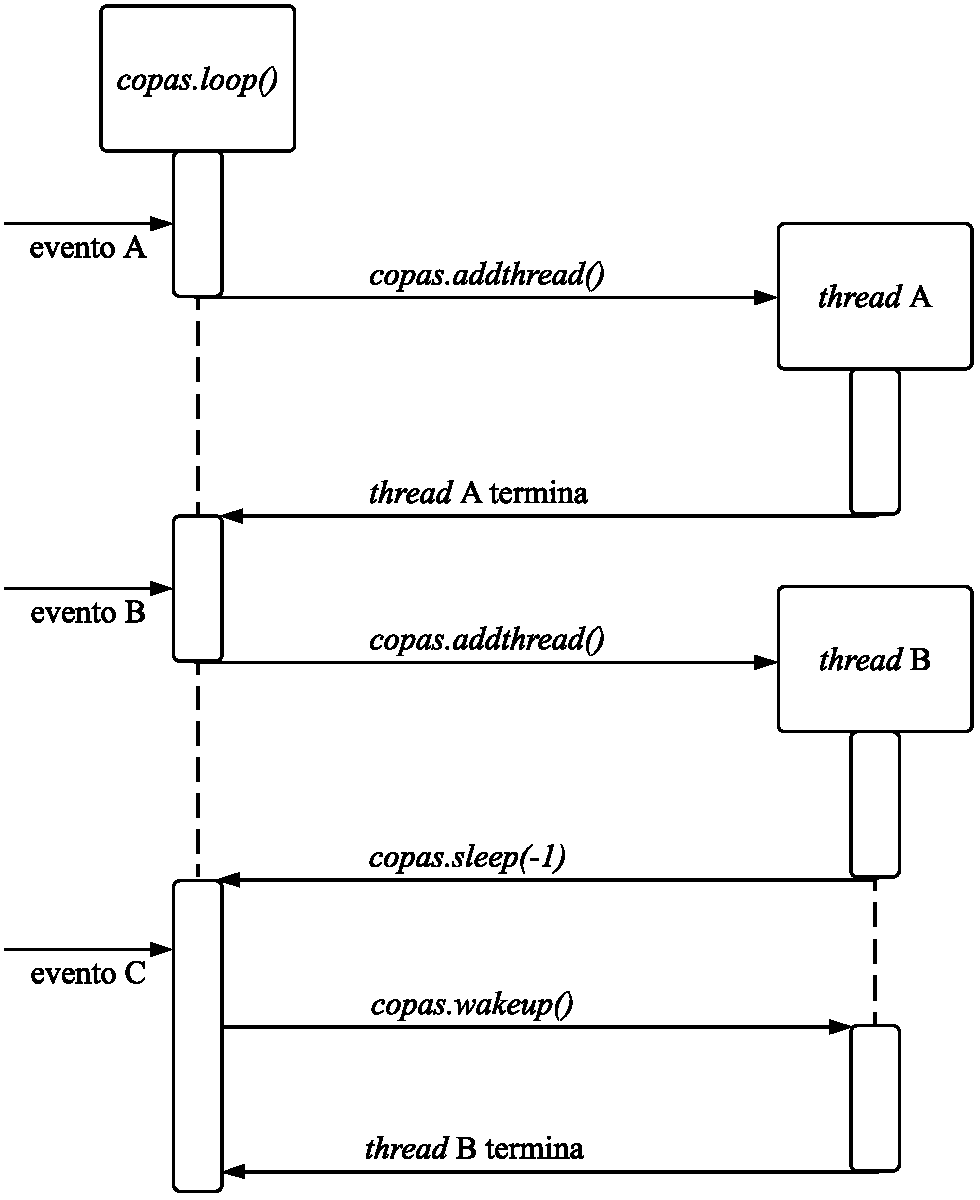
\includegraphics[width=0.8\textwidth]{./fig/events}
 \caption{Diagrama de sequência UML que modela a programação orientada a eventos utilizando a biblioteca Copas.}
 \label{fig:events}
\end{figure}

\section{Modelo de Concorrência}

O modelo de programação concorrente também foi necessário para atender aos requisitos de um cliente HTTP/2. Conforme visto na Seção \ref{subsec:fluxos}, um servidor pode multiplexar fluxos em uma única conexão HTTP/2. Isso significa que múltiplos fluxos podem estar sendo enviados pelo servidor de modo concorrente em qualquer momento durante uma conexão HTTP/2. Precisamos então de uma espécie de escalonador de fluxos para que possamos lidar com múltiplos fluxos sendo enviados concorrentemente por um servidor HTTP/2. 

Para recebermos e processarmos fluxos concorrentes, também precisamos de operações assíncronas ao nível de {\em sockets} TCP porque o modelo clássico de bloquear operações de rede não resolve o problema de tratar fluxos concorrentes na conexão TCP (que na verdade são apenas uma cadeia de bytes dentro do {\em buffer} TCP), além de ser uma abordagem ineficiente porque o cliente passaria a maior parte do tempo bloqueado na chamada de rede {\em receive} do {\em socket}.

Visando obter tanto concorrência para processar fluxos quanto operações de rede assíncronas, também utilizamos a biblioteca Copas. Nesse caso, o objetivo de Copas é escalonar múltiplos fluxos que podem estar presentes dentro da conexão TCP. As funcionalidades de Copas de prover operações assíncronas, descritas na Seção \ref{subsec:copas}, atendem bem o papel de escalonar os fluxos no nível de {\em sockets} TCP por combinar as características de {\em multithreading} cooperativa de Lua com as operações assíncronas de rede da biblioteca LuaSocket \cite{Nehab2007}.

Sempre que o {\em dispatcher} de Copas verifica que uma {\em thread} ainda está realizando alguma operação de rede {\em receive}, mas ainda não a concluiu, o {\em status} identificado por ``{\em timeout}'' de LuaSocket é sinalizado, o que significa que a operação retornou por incompleto. Nesse caso, a {\em thread} é suspensa por Copas. Internamente, o {\em dispatcher} de Copas implementa um {\em loop} despachante que emprega um mecanismo de notificação para obter o resultado do processamento de alguma operação de rede assíncrona contida em {\em threads} distintas, chamando uma por uma.

Assim, antes de detalharmos a implementação de ambos os modelos vistos e como eles foram empregados para implementar o lado cliente do HTTP/2, a Figura \ref{fig:deps} formaliza as dependências da biblioteca http2 através de um diagrama de componentes UML, em que cada biblioteca é representada por um componente. A biblioteca http2 depende da biblioteca LuaSocket para obter suporte tanto ao protocolo TCP quanto a funcionalidades de construção e processamento de URLs; de Copas para construirmos um escalonador de fluxos e obtermos operações de rede assíncronas e de LuaSec \cite{silvestre2018luasec} para fazer uso de conexões TLS seguras através do protocolo ALPN \cite{FriedlRFC7301}. Na próxima seção mostramos outro diagrama de componentes UML que ilustra a estrutura interna da biblioteca http2.

\begin{figure}[hbt!]
 \centering
  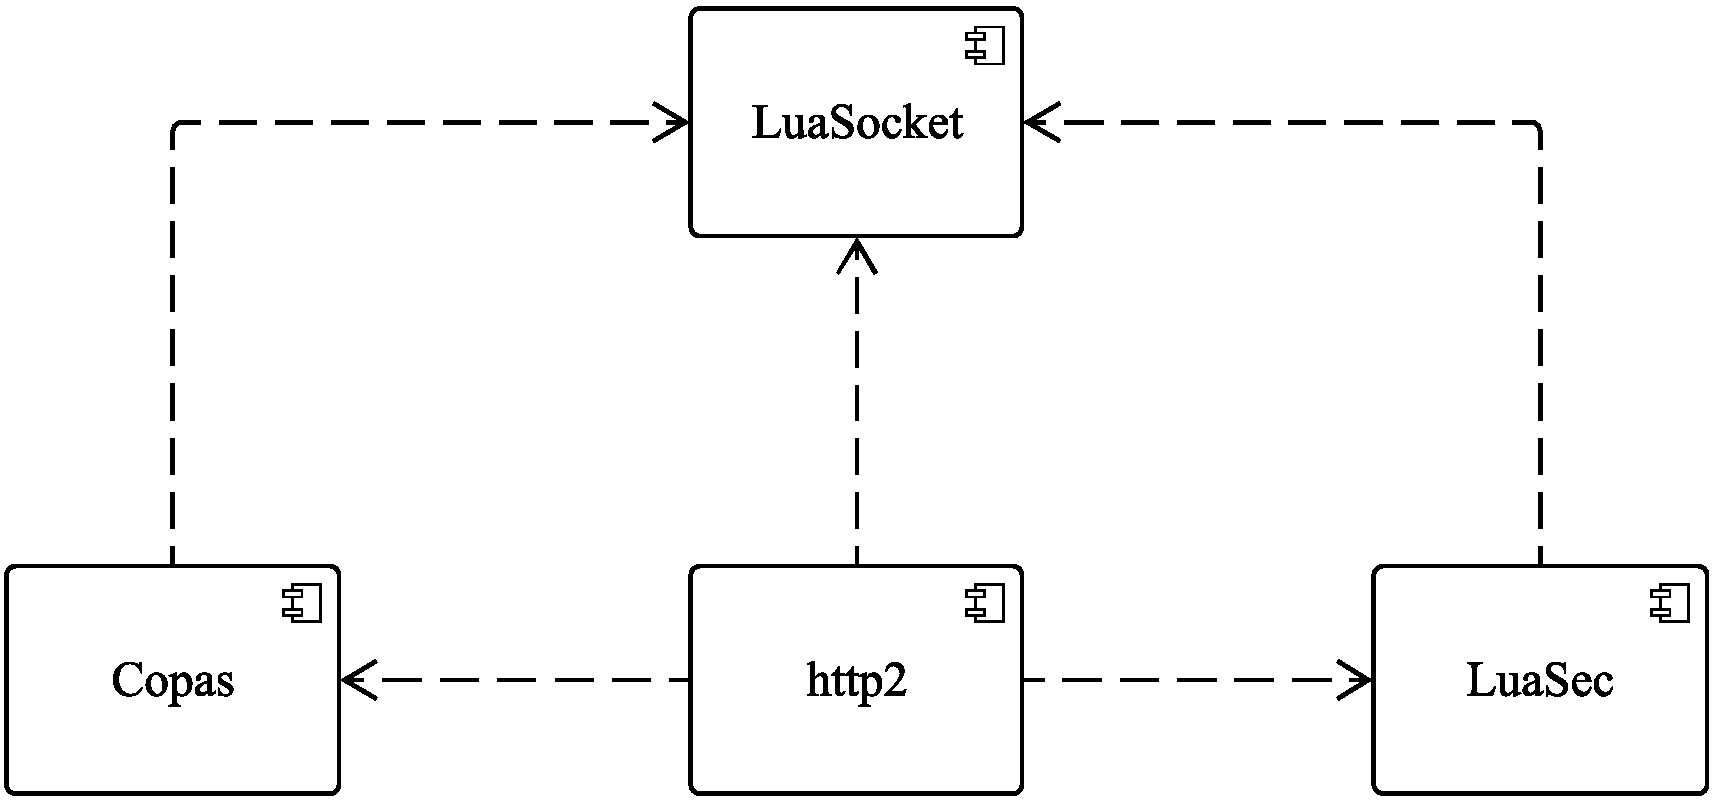
\includegraphics[width=\textwidth]{./fig/deps}
 \caption{Dependências da biblioteca http2 por outras bibliotecas de Lua.}
 \label{fig:deps}
\end{figure}

\section{Modelagem do Código-fonte}
\label{sec:components}

O diagrama de componentes UML retratado na Figura \ref{fig:deps} mostra como o código-fonte da biblioteca http2 foi modelado. O programador apenas interage com o módulo {\em http2} diretamente, sendo que os demais servem para oferecer interfaces projetadas especificamente em torno do suporte para as características de baixo nível do protocolo HTTP/2, além de permitir uma melhor organização de código através da modularização de funcionalidades.

\begin{itemize}
    \item {\em connection}: encapsula o gerenciamento de uma conexão HTTP/2.
    \item {\em stream}: encapsula o gerenciamento de fluxos HTTP/2.
    \item {\em framer}: realiza codificação e decodificação de quadros HTTP/2.
    \item {\em hpack}: realiza a codificação e decodificação de campos de cabeçalhos.
    \item {\em http2}: oferece a interface necessária para a criação de um cliente HTTP/2.
\end{itemize}

\begin{figure}[hbt!]
 \centering
  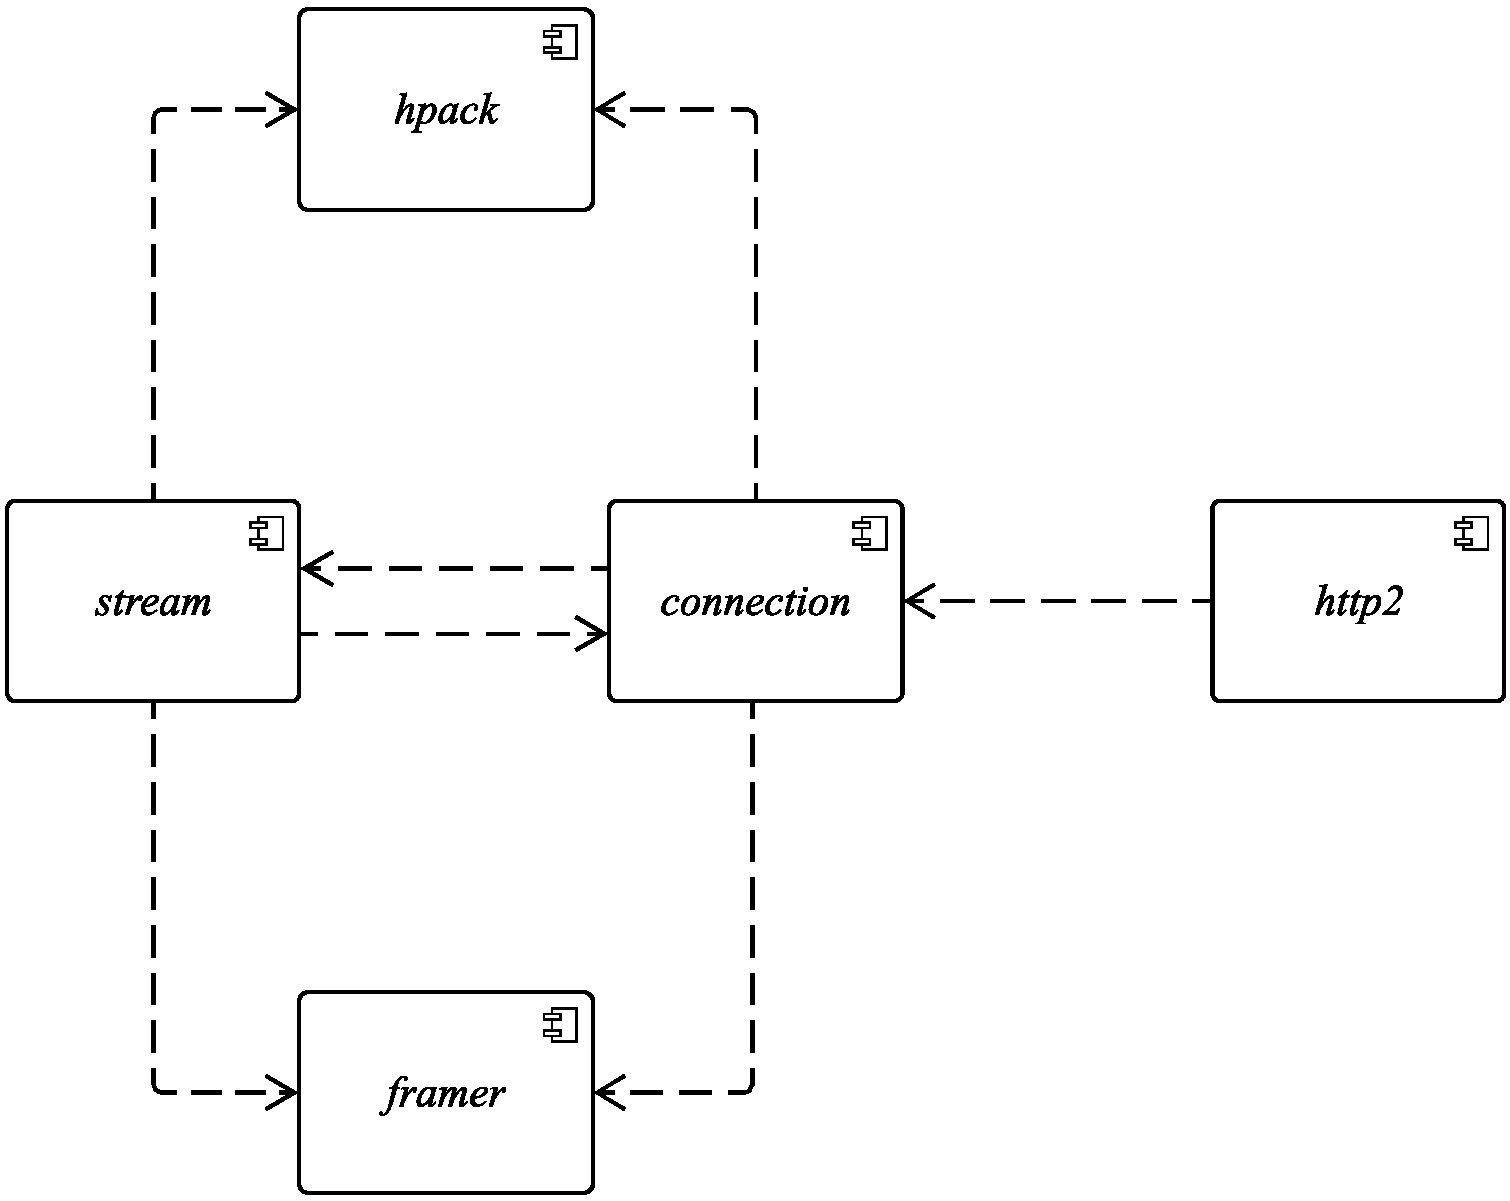
\includegraphics[width=\textwidth]{./fig/source}
 \caption{Componentes da biblioteca http2.}
 \label{fig:source}
\end{figure}

\subsection{Módulo {\em connection}}
\label{subsec:connection}

Alguns quadros HTTP/2 como {\em WINDOW\_UPDATE}, {\em SETTINGS} e {\em GOAWAY} são enviados a nível de uma conexão HTTP/2 e são pertinentes à toda sessão de comunicação entre clientes e servidores. No HTTP/2, é adotado a convenção de que esses quadros são enviados em um fluxo com identificador 0, indicando que esse fluxo é reservado para controlar a conexão e não pode ser utilizado para criar outros fluxos. Para tanto, o módulo {\em connection} foi criado para abstrair a responsabilidade de controlar uma conexão do módulo de fluxos {\em stream} (ver Seção \ref{subsec:stream}).

Essencialmente, o módulo {\em connection} oferece toda a lógica necessária para um cliente HTTP/2 se comportar com as exigências especificadas de um cliente HTTP/2 em termos do uso que ele faz da conexão HTTP/2 \footnote{Na verdade, esse comportamento é simétrico entre clientes e servidores, ou seja, as mesmas funcionalidades do módulo {\em connection} podem ser aplicadas tanto para clientes quanto para servidores HTTP/2.}. As funções disponibilizadas por esse módulo são:

\begin{itemize}
    \item \verb|connection:window_update(payload)|: envia um quadro {\em WINDOW\_UPDATE} com o seu respectivo corpo (\verb|payload|) para o servidor.
    \item \verb|connection:settings(payload)|: envia um quadro {\em SETTINGS} com o seu respectivo corpo (\verb|payload|) para o servidor.
    \item \verb|connection:goaway(payload)|: envia um quadro {\em GOAWAY} com o seu respectivo corpo (\verb|payload|) para o servidor.
    \item \verb|connection:parse_stream()|: encapsula toda a funcionalidade requerida para decodificar e processar um fluxo HTTP/2 contido no {\em buffer} do TCP.
    \item \verb|connection:new_stream(identifier)|: aloca e retorna um novo fluxo (\verb|stream|) para a conexão atual atribuindo-lhe o identificador \verb|identifier|.
    \item \verb|connection:new()|: construtor para uma nova conexão HTTP/2.
\end{itemize}

\subsection{Módulo {\em stream}}
\label{subsec:stream}

Uma única conexão HTTP/2 pode multiplexar múltiplos fluxos concorrentes: múltiplas requisições e respostas podem ser enviadas simultaneamente e os dados (quadros) do fluxo podem ser intercalados e priorizados. O módulo {\em stream} encapsula todo o gerenciamento de estados, transições, controle de fluxo e gerenciamento de erros no nível de fluxos conforme definidos pela especificação do HTTP/2. As funções disponibilizadas por esse módulo são:

\begin{itemize}
    \item \verb|stream:parse(frame)|: processa um quadro (\verb|frame|) proveniente de um fluxo HTTP/2.
    \item \verb|stream:headers(payload)|: envia um quadro {\em HEADERS} com o seu respectivo corpo (\verb|payload|) para o servidor.
    \item \verb|stream:window_update(payload)|: envia um quadro {\em WINDOW\_UPDATE} com o seu respectivo corpo (\verb|payload|) para o servidor.
    \item \verb|stream:new()|: construtor para um novo fluxo HTTP/2.
\end{itemize}

\subsection{Módulo {\em framer}}
\label{subsec:framer}

Como visto na Seção \ref{subsec:framing}, uma das melhorias trazidas pelo HTTP/2 em relação ao HTTP/1.1 é a forma como as mensagens HTTP são codificadas e decodificadas para serem enviadas na conexão TCP. No HTTP/2, cada mensagem HTTP/1 é mapeada para um quadro, a unidade de comunicação básica do HTTP/2, com o intuito de introduzir um novo enquadramento binário de mensagens. O módulo {\em framer} (``enquadrador'') implementa esse novo enquadramento, cuja função é descrever a maneira que quadros HTTP/2 são estruturados para serem formados em fluxos multiplexados. As funções auxiliares providas por esse módulo são:

\begin{itemize}
    \item \verb|encode(frame)|: gera um quadro HTTP/2 codificado em binário a partir de suas características desejáveis (cabeçalho e corpo) passadas como parâmetro (\verb|frame|).
    \item \verb|decode(buffer)|: decodifica um quadro HTTP/2 completo a partir de um \verb|buffer| TCP passado como parâmetro e retorna os campos referentes ao cabeçalho e ao corpo desse quadro.
\end{itemize}

\subsection{Módulo {\em hpack}}
\label{subsec:hpack}

A implementação do formato de compressão de cabeçalhos para o HTTP/2 (HPACK) \cite{BelsheRFC7541} para representar os cabeçalhos HTTP mais eficientemente é fornecido pelo módulo {\em hpack}. Apenas as funções utilitárias de codificação e decodificação de cabeçalhos foram implementadas nesse módulo, que são:

\begin{itemize}
    \item \verb|encode(header_list)|: responsável por codificar listas de pares chave-valor (\verb|header_list|) utilizando o algoritmo HPACK.
    \item \verb|decode(header_block)|: processa um bloco de cabeçalhos (\verb|header_block|).
    \item \verb|new(HEADER_TABLE_SIZE)|: cria e retorna um novo contexto HPACK a partir do parâmetro do quadro {\em SETTINGS}, \verb|HEADER_TABLE_SIZE|.
\end{itemize}

\begin{center}
 \begin{minipage}{0.7\textwidth}
  \begin{codigo}[H]
   \small
   \VerbatimInput[xleftmargin=10mm,numbers=left,obeytabs=true]{./prog/client.lua}
   \caption{\texttt{Cliente HTTP/2}}
   \label{code:client}
  \end{codigo}
 \end{minipage}
\end{center}

\subsection{Módulo {\em http2}}
\label{subsec:http2lua}

Talvez o módulo mais importante da implementação seja o {\em http2}, que merece atenção especial nesta seção. Trata-se de um módulo responsável por prover ao programador operações específicas de um cliente HTTP/2, bem como controlar o fluxo de execução do {\em loop} de eventos do Copas. Como o modelo de programação da biblioteca http2 é orientado a eventos, o código do programador é encarregado de tratar um evento emitido durante a sessão de comunicação com um servidor HTTP/2.

Para melhor expor o funcionamento desse módulo, considere um exemplo de um código cliente HTTP/2 que faz uso da biblioteca http2, ilustrado no Código \ref{code:client}. Nesse código, o programador registrou algumas funções anônimas atuando como funções de {\em callback} para tratarem de determinados eventos.

\begin{itemize}
    \item Na linha 5, uma função é registrada como tratadora do evento {\em on\_connect}, que é emitido quando uma conexão HTTP/2 com o servidor é estabelecida. Essa função de {\em callback} é invocada com o argumento \verb|session|, que representa uma sessão de comunicação HTTP/2 com o servidor.
    \item Na linha 6, uma requisição é submetida ao servidor conectado através da função \verb|request|. Essa requisição é realizada enviando cabeçalhos padrões definidos pela biblioteca, pois nenhum argumento foi passado para a função \verb|request|.
    \item Na linha 8, uma função é registrada como tratadora do evento {\em on\_response}, que é emitido quando um quadro {\em HEADERS} é recebido do servidor HTTP/2 conectado do fluxo correspondente à requisição \verb|req|. Essa função de {\em callback} é invocada com o argumento \verb|headers|, que contém o objeto que representa cabeçalhos HTTP/2 (uma tabela bidimensional de listas de cabeçalhos).
    \item Na linha 16, uma função é registrada como tratadora do evento {\em on\_data}, que é emitido quando o servidor HTTP/2 conectado termina de enviar dados (através de quadros {\em DATA}). Essa função de {\em callback} é invocada com o argumento \verb|data|, que é uma variável do tipo string contendo os dados transmitidos pelo servidor.
\end{itemize}

O Código \ref{code:client} pode ser facilmente estendido para realizar mais de uma requisição, bastando apenas repetir as chamadas de funções e trocando os nomes das variáveis associadas a requisição. Nesse contexto, o papel do módulo {\em http2} é abstrair o enquadramento de mensagens e multiplexação de fluxos de baixo nível realizados pela biblioteca, permitindo que o programador se concentre apenas na lógica de sua aplicação ou de seu cliente específico desde que as funções da API sejam corretamente chamadas.

As funções de alto nível fornecidas pelo módulo {\em http2} representam eventos que são emitidos quando computações específicas sobre dados transmitidos pelo servidor são enviados. Esses dados são passados como argumentos para as funções de {\em callback} registradas pelo programador para que ele possa tratá-los apropriadamente. Efetivamente, essas funções compõem a API da biblioteca http2 e são explicadas na Seção \ref{sec:api}. Uma função de baixo nível que faz parte da estrutura interna do módulo {\em http2} é chamada de {\em dispatcher} e é explicada em seguida.

\subsubsection{{\em Dispatcher}}

O {\em dispatcher} é uma função interna do módulo {\em http2} e é uma parte importante na biblioteca http2, pois ele é o responsável por realizar a tarefa de intercalar os quadros contidos em diferentes fluxos concorrentemente abertos em uma conexão TCP, bem como despachar {\em threads} associadas a esses fluxos. Ele foi construído baseando-se no modelo de programação concorrente com as características descritas nas Seções \ref{subsec:coroutines} e \ref{subsec:copas} e também no modelo de programação orientado a eventos com as características descritas no início deste capítulo.

Essencialmente, o {\em dispatcher} é um simples {\em loop} que recebe um quadro de um {\em buffer} TCP, determina a que fluxo esse quadro pertence e processa o seu conteúdo para que ele possa ser adequadamente intercalado. Como os fluxos HTTP/2 são concorrentes entre si, fica a cargo do {\em dispatcher} administrar esse nível de concorrência de modo a evitar problemas de coordenação e sincronização. Intercalado um quadro, o {\em dispatcher} verifica se alguma {\em thread} pode ser acordada em resposta ao término do processamento de determinados quadros de um fluxo.

É mais fácil entender o {\em dispatcher} visualizando seu código. O Código \ref{code:dispatcher} mostra como a implementação do {\em dispatcher} foi feita em função do gerenciamento de {\em threads} do Copas e do ciclo de vida um fluxo. Com o auxílio da função \verb|connection:parse_stream| (ver Seção \ref{sec:components}, intercalamos quadros HTTP/2 contidos em um fluxo específico. Através do {\em dispatcher}, o ciclo de vida de um fluxo (mostrado na Figura \ref{fig:ciclo_fluxo}) é efetivamente implementado. Observamos que esse ciclo de vida foi implementado utilizando o modelo de programação orientada a eventos: quando um determinado estado de um fluxo é alcançado, despachamos a {\em thread} (nesse caso, a {\em callback}) que trata desse estado com a função \verb|copas.wakeup|. O {\em loop} termina quando o estado {\em closed} é alcançado.

\section{API}
\label{sec:api}

A API da biblioteca http2 é definida em termos do modelo de programação orientada a eventos com as características descritas no início deste capítulo. O Código \ref{code:client} serve como um exemplo da maneira que o programador pode utilizar a biblioteca chamando funções da API disponibilizada. Todas as funções da API são definidas da seguinte forma:

\begin{itemize}
    \item \verb|http2.on_connect(url, callback)|: dispara a função de resposta \verb|callback| quando uma conexão HTTP/2 é estabelecida com o servidor identificado por \verb|url|. Retorna uma tabela representando uma sessão de comunicação HTTP/2.
    \item \verb|session.request([headers, body])|: submete uma requisição para o servidor HTTP/2 conectado na sessão \verb|session| e retorna uma tabela utilizada para invocar funções de {\em callback} associadas a essa requisição (vê-las a seguir). Caso estejam presentes, \verb|headers| é uma tabela bidimensional contendo listas de cabeçalhos HTTP/2 e \verb|body| é o corpo de uma requisição POST. Caso contrário, uma requisição GET é submetida com campos de cabeçalhos extraídos da URL passada como argumento da função \verb|on_connect|.
    \item \verb|req.on_response(callback)|: dispara a função de resposta \verb|callback| quando um quadro {\em HEADERS} é recebido do servidor HTTP/2 conectado do fluxo correspondente à requisição \verb|req|. A função \verb|callback| é invocada com uma tabela bidimensional contendo listas de cabeçalhos HTTP/2.
    \item \verb|req.on_data(callback)|: dispara a função de resposta \verb|callback| quando o servidor HTTP/2 conectado termina de enviar dados (através de quadros {\em DATA}). A função \verb|callback| é invocada com uma string contendo os valores dos dados recebidos.
\end{itemize}

\begin{center}
 \begin{minipage}{0.7\textwidth}
  \begin{codigo}[H]
   \small
   \VerbatimInput[xleftmargin=10mm,numbers=left,obeytabs=true]{./prog/dispatcher.lua}
   \caption{\texttt{Dispatcher}}
   \label{code:dispatcher}
  \end{codigo}
 \end{minipage}
\end{center}

\section{Considerações Finais}
\label{sec:implfinals}

O presente capítulo descreveu a implementação da biblioteca http2. O código-fonte, juntamente com o cliente mostrado na Seção \ref{fig:source} podem ser encontrados em \cite{Paulahttp2}. Requisições simples com os métodos de requisição {\em GET} e {\em POST} estão funcionando e foram testadas (outros métodos como {\em HEAD} e {\em PUT} podem ser simulados a partir desses dois), embora somente o HTTP/2 executado sobre uma conexão TLS seja suportado por padrão. Essa decisão foi tomada em reflexo da tendência atual de habilitar TLS por padrão tanto em navegadores quanto servidores e devido à pouca utilização do protocolo HTTP/2 sobre o TCP puro.

Como a implementação foi inteiramente escrita na linguagem Lua, alcançamos a capacidade de multiplataforma da biblioteca http2 porque Lua é uma linguagem multiplataforma. Com isso, a biblioteca segue a portabilidade de Lua. Uma restrição importante da implementação é que a biblioteca http2 não é compatível com versões anteriores à versão 5.3 de Lua. Essa decisão foi tomada sobretudo com base nas facilidades de manipulação de bits dessa versão e também visando a simplicidade da implementação.

Visto que o HTTP/2 é um protocolo extenso e complexo em funcionalidades, a biblioteca http2 oferece um suporte mínimo necessário para implementar as características básicas de um cliente HTTP/2. O programador não precisa ter total conhecimento do ciclo de vida de um fluxo porque atualmente apenas requisições simples podem ser feitas, ou seja, os estados e as transições que ocorrem na visão do programador são controlados internamente pela biblioteca. Na visão da biblioteca, contudo, implementamos os estados ocioso, aberto, semifechado (remoto) e fechado.

Como resultado, as principais características de um cliente HTTP/2 foram implementadas, como a habilidade de realizar multiplexação de fluxos e de fazer compressão e descompressão de campos de cabeçalhos. Em termos das outras novas características do HTTP/2, o {\em push} de requisições\slash respostas do servidor e priorizações de requisições não foram implementados, uma vez que o HTTP/2 não obriga o suporte para ambos esses mecanismos e também devido à limitação de tempo disponível para implementar essas novidades. Consequentemente, quadros {\em PRIORITY} e {\em PUSH\_PROMISE} não foram implementados. O quadro {\em PING} também não foi implementado porque ainda não mantemos verificações periódicas sobre o estado da conexão. Os outros quadros foram implementados e são suportados por padrão.